\documentclass[10pt,landscape]{article}
\usepackage{multicol}
\usepackage{calc}
\usepackage{ifthen}
\usepackage[landscape]{geometry}
\usepackage{hyperref}

\usepackage[OT1]{fontenc}
\usepackage[sc]{mathpazo}
\usepackage[utf8]{inputenc}
\usepackage[german]{babel}
\usepackage{amsmath}
\usepackage{amsfonts}
\usepackage{amssymb}
\usepackage{mathtools}
\usepackage{fancyhdr}
\usepackage{setspace}
\usepackage{listings}
\usepackage{stmaryrd}
\usepackage{graphicx}
\usepackage{changepage}
\usepackage{enumitem}
\usepackage{wrapfig}
\usepackage{tikz} 
\usepackage{xcolor, soul}
\newcommand{\green}[1]{\sethlcolor{green}\hl{#1}}
\newcommand{\yellow}[1]{\sethlcolor{yellow} \hl{#1}}
\newcommand{\blue}[1]{\sethlcolor{cyan} \hl{#1}}


% To make this come out properly in landscape mode, do one of the following
% 1.
%  pdflatex latexsheet.tex
%
% 2.
%  latex latexsheet.tex
%  dvips -P pdf  -t landscape latexsheet.dvi
%  ps2pdf latexsheet.ps


% If you're reading this, be prepared for confusion.  Making this was
% a learning experience for me, and it shows.  Much of the placement
% was hacked in; if you make it better, let me know...


% 2008-04
% Changed page margin code to use the geometry package. Also added code for
% conditional page margins, depending on paper size. Thanks to Uwe Ziegenhagen
% for the suggestions.

% 2006-08
% Made changes based on suggestions from Gene Cooperman. <gene at ccs.neu.edu>


% To Do:
% \listoffigures \listoftables
% \setcounter{secnumdepth}{0}


% This sets page margins to .5 inch if using letter paper, and to 1cm
% if using A4 paper. (This probably isn't strictly necessary.)
% If using another size paper, use default 1cm margins.
\ifthenelse{\lengthtest { \paperwidth = 11in}}
	{ \geometry{top=.5in,left=.5in,right=.5in,bottom=.5in} }
	{\ifthenelse{ \lengthtest{ \paperwidth = 297mm}}
		{\geometry{top=1cm,left=1cm,right=1cm,bottom=1cm} }
		{\geometry{top=1cm,left=1cm,right=1cm,bottom=1cm} }
	}

% Turn off header and footer
\setcounter{page}{1}


% Redefine subsection commands to use less space
\makeatletter
\renewcommand{\subsection}{\@startsection{subsection}{1}{0mm}%
                                {-1ex plus -.5ex minus -.2ex}%
                                {0.5ex plus .2ex}%x
                                {\normalfont\large\bfseries}}
\renewcommand{\subsection}{\@startsection{subsection}{2}{0mm}%
                                {-1explus -.5ex minus -.2ex}%
                                {0.5ex plus .2ex}%
                                {\normalfont\normalsize\bfseries}}
\renewcommand{\subsubsection}{\@startsection{subsubsection}{3}{0mm}%
                                {-1ex plus -.5ex minus -.2ex}%
                                {1ex plus .2ex}%
                                {\normalfont\small\bfseries}}
\makeatother

% Define BibTeX command
\def\BibTeX{{\rm B\kern-.05em{\sc i\kern-.025em b}\kern-.08em
    T\kern-.1667em\lower.7ex\hbox{E}\kern-.125emX}}

% Don't print subsection numbers
\setcounter{secnumdepth}{0}


\setlength{\parindent}{0pt}
\setlength{\parskip}{0pt plus 0.5ex}


% -----------------------------------------------------------------------

\begin{document}
\raggedright
\footnotesize
\begin{multicols}{3}


% multicol parameters
% These lengths are set only within the two main columns
%\setlength{\columnseprule}{0.25pt}
\setlength{\premulticols}{1pt}
\setlength{\postmulticols}{1pt}
\setlength{\multicolsep}{1pt}
\setlength{\columnsep}{2pt}

\begin{center}
     \Large{\textbf{WuS - Cheatsheet}} \\
\end{center}
\section{Wahrscheinlichkeitsräume}
\subsection{Grundraum}
\blue{Terminologie:} Die Menge $\Omega$ nennen wir Grundraum. 
\subsection{Ereignisse}
Ein Element $\omega \in \Omega$ nennen wir Elementarereignis (oder Ausgang des Experiments).\\
\blue{Definition 1.1:} Ein Mengensystem $\mathcal{F} \subset \mathcal{P}(\Omega)$ heisst Sigma-Algebra ( $\sigma$-Algebra), falls es die folgenden Eigenschaften erfüllt
\begin{enumerate}
    \item $\Omega \in \mathcal{F}$
    \item $A \in \mathcal{F} \Rightarrow A^{c} \in \mathcal{F}$ 
    \item $A_{1}, A_{2}, \ldots \in \mathcal{F} \Rightarrow \bigcup_{i=1}^{\infty} A_{i} \in \mathcal{F}$
\end{enumerate}
Dabei nennen wir die Elemente der $\sigma$-Algebra Ereignisse.\\
\subsection{Wahrscheinlichkeitsmass}
\blue{Definition 1.2:} Sei $\Omega$ ein Grundraum und sei $\mathcal{F}$ eine $\sigma$-Algebra. Eine Abbildung
$$
\begin{aligned}
\mathbb{P}: \mathcal{F} & \rightarrow[0,1] \\
A & \mapsto \mathbb{P}[A]
\end{aligned}
$$
heisst Wahrscheinlichkeitsmass auf $(\Omega, \mathcal{F})$, falls folgende Eigenschaften gelten
\begin{enumerate}
    \item $\mathbb{P}[\Omega]=1$.
    \item ( $\sigma$-Additivität) $\mathbb{P}[A]=\sum_{i=1}^{\infty} \mathbb{P}\left[A_{i}\right] \quad$ if $A=\bigcup_{i=1}^{\infty} A_{i}$ (disjunkte Vereinigung).
\end{enumerate}
\subsection{Der Wahrscheinlichkeitsraum} 
\blue{Definition 1.3:} Sei $\Omega$ ein Grundraum, $\mathcal{F}$ eine $\sigma$-Algebra, und $\mathbb{P}$ ein Wahrscheinlichkeitsmass. Wir nennen das Tripel $(\Omega, \mathcal{F}, \mathbb{P})$ Wahrscheinlichkeitsraum.\\
\textbf{Bemerkung 1.4:} Das Ereignis $A=\varnothing$ tritt niemals ein. Das Ereignis $A=\Omega$ tritt stets ein.\\
\blue{Definition 1.5:} Sei $\Omega$ eine endlicher Grundraum. Das Laplace Modell auf $\Omega$ ist ein Tripel $(\Omega, \mathcal{F}, \mathbb{P})$, sodass
\begin{enumerate}
    \item $\mathcal{F}=\mathcal{P}(\Omega)$,
    \item  $\mathbb{P}: \mathcal{F} \rightarrow[0,1]$ ist definiert durch
    $$
    \forall A \in \mathcal{F} \quad \mathbb{P}[A]=\frac{|A|}{|\Omega|} .
    $$
\end{enumerate}
\subsection{Eigenschaften von Ereignissen}
\yellow{Satz 1.6 (Abgeschlossenheit der $\sigma$-Algebra bzgl. Operationen):} Sei $\mathcal{F}$ eine $\sigma$-Algebra auf $\Omega$. Es gilt
\begin{enumerate}
    \item $\varnothing \in \mathcal{F}$,
    \item $A_{1}, A_{2}, \ldots \in \mathcal{F} \Rightarrow \bigcap_{i=1}^{\infty} A_{i} \in \mathcal{F}$,
    \item $A, B \in \mathcal{F} \Rightarrow A \cup B \in \mathcal{F}$,
    \item $A, B \in \mathcal{F} \Rightarrow A \cap B \in \mathcal{F}$.
\end{enumerate}
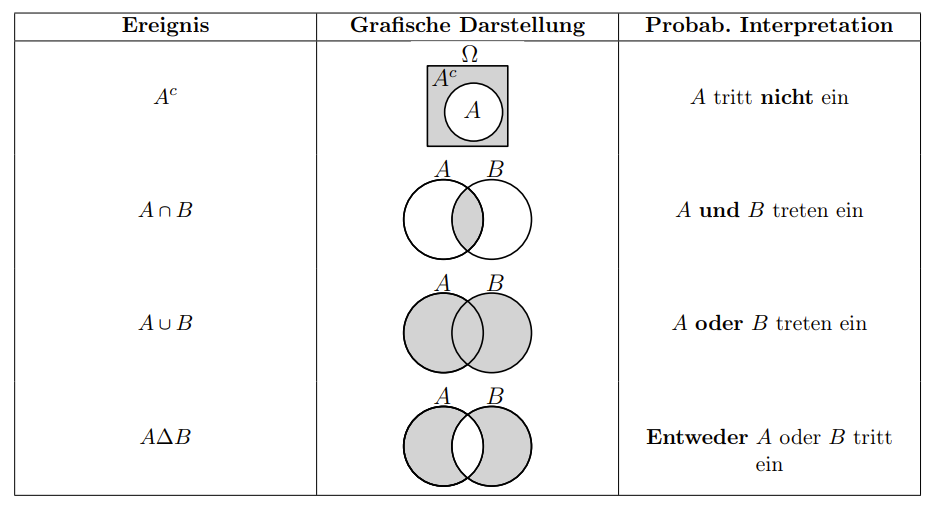
\includegraphics[width = 0.3\textwidth]{prob_interpr_sets.png}
\textbf{Beziehung/Interpretationen zwischen Ereignissen}
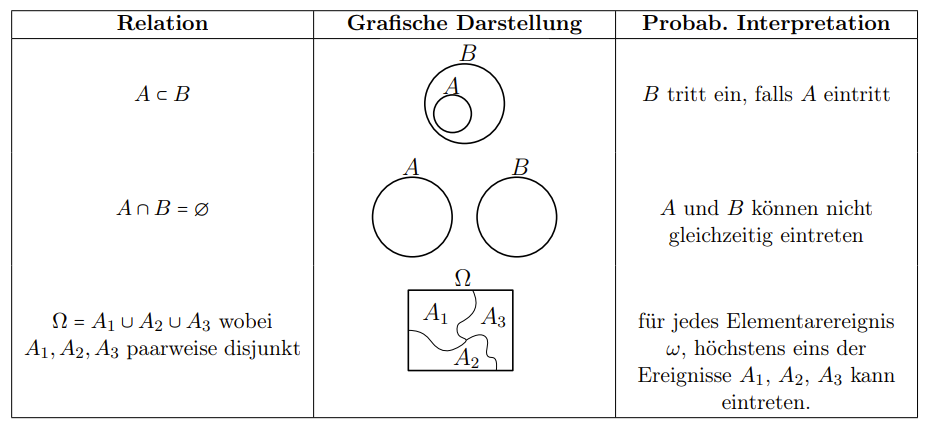
\includegraphics[width = 0.3\textwidth]{prob_interpr_two_events.png}
\subsection{Eigenschaften von Wahrscheinlichkeitsmassen}
\yellow{Satz 1.7:} Sei $\mathbb{P}$ ein Wahrscheinlichkeitsmass auf $(\Omega, \mathcal{F})$. Es gilt:
\begin{enumerate}
    \item $\mathbb{P}[\varnothing]=0$
    \item (Additivität) Sei $k \geq 1$, seien $A_{1}, \ldots, A_{k}$-viele paarweise disjunkte Ereignisse, dann gilt 
    $$
    \mathbb{P}\left[A_{1} \cup \cdots \cup A_{k}\right]=\mathbb{P}\left[A_{1}\right]+\cdots+\mathbb{P}\left[A_{k}\right]
    $$
    \item Sei $A$ ein Ereignis, dann gilt $\mathbb{P}\left[A^{c}\right]=1-\mathbb{P}[A]$
    \item Falls $A$ und $B$ zwei (nicht notwendigerweise disjunkte) Ereignisse, dann gilt 
    $$
    \mathbb{P}[A \cup B]=\mathbb{P}[A]+\mathbb{P}[B]-\mathbb{P}[A \cap B]
    $$
\end{enumerate}
\subsection{Nützliche Ungleichungen}
\yellow{Satz $1.8$ (Monotonie):} Seien $A, B \in \mathcal{F}$, dann gilt $A \subset B \Rightarrow \mathbb{P}[A] \leq \mathbb{P}[B].$\\
\yellow{Satz $1.9$ (Union Bound):} Sei $A_{1}, A_{2}, \ldots$ eine Folge von (nicht notwendigerweise disjunkten) Ereignissen, dann gilt die folgende Ungleichung
$\mathbb{P}\left[\bigcup_{i=1}^{\infty} A_{i}\right] \leq \sum_{i=1}^{\infty} \mathbb{P}\left[A_{i}\right]$.\\
\textbf{Bemerkung 1.10:} Die obrige Ungleichung gilt ebenfalls für eine Folge von endlich vielen nicht-leeren Ereignissen.
\subsection{Stetigkeit von Wahrscheinlichkeitsmassen}
\yellow{Satz 1.11:} Sei $\left(A_{n}\right)$ eine monoton wachsende Folge von Ereignissen $\left(\forall n: A_{n} \subset A_{n+1}\right).$ Dann gilt
$$
\lim _{n \rightarrow \infty} P\left[A_{n}\right]=\mathbb{P}\left[\bigcup^{\infty} A_{n}\right] . \quad \text { monoton wachsender Grenzwert }
$$
Sei $\left(B_{n}\right)$ eine monoton fallende Folge von Ereignissen $\forall n: \left(B_{n} \supset B_{n+1}\right).$ Dann gilt
$$
\lim _{n \rightarrow \infty} P\left[B_{n}\right]=\mathbb{P}\left[\bigcap_{n=1}^{\infty} B_{n}\right] . \quad \text { monoton fallender Grenzwert }
$$.\\
\textbf{Bemerkung 1.12:} Durch Monotonie erhalten wir $\mathbb{P}\left[A_{n}\right] \leq \mathbb{P}\left[A_{n+1}\right]$ und $\mathbb{P}\left[B_{n}\right] \geq \mathbb{P}\left[B_{n+1}\right]$ für jedes n. 
Daher sind die Grenzwerte in den obrigen Gleichungen wohldefiniert.
\subsection{Bedingte Wahrscheinlichkeit}
\blue{Definition $1.13$ (Bedingte Wahrscheinlichkeit):} Sei $(\Omega, \mathcal{F}, \mathbb{P})$ ein Wahrscheinlichkeitsraum. Seien $A, B$ zwei Ereignisse mit $\mathbb{P}[B]>0$. Wir definieren die bedingte Wahrscheinlichkeit von $A$ gegeben $B$ wie folgt
$$
\mathbb{P}[A \mid B]=\frac{\mathbb{P}[A \cap B]}{\mathbb{P}[B]} .
$$\\
\textbf{Bemerkung 1.14:} $\mathbb{P}[B \mid B]=1$.\\
\yellow{Satz 1.15:} Sei $(\Omega, \mathcal{F}, \mathbb{P})$ ein Wahrscheinlichkeitsraum. Sei $B$ ein Ereignis mit positiver Wahrscheinlichkeit. 
Dann ist $\mathbb{P}[. \mid B]$ ein $W$-Mass auf $\Omega$.\\
\yellow{Satz $1.16$ (Gesetz der totalen Wahrscheinlichkeit):} Sei $B_{1}, \cdots, B_{n}$ $\text{eine Partition}^{a}$ des Grundraums $\Omega$, so dass $\mathbb{P}\left[B_{i}\right]>0$ für jedes $1 \leq i \leq n$ gilt. Dann gilt
$$
\forall A \in \mathcal{F} \quad \mathbb{P}[A]=\sum_{i=1}^{n} \mathbb{P}\left[A \mid B_{i}\right] \mathbb{P}\left[B_{i}\right]
$$
$a_{\text{i.e. }} \Omega=B_{1} \cup \cdots \cup B_{n}$ mit paarweise disjunkten Ereignissen. \\
\yellow{Satz $1.17$ (Satz von Bayes):} Sei $B_{1}, \ldots, B_{n} \in \mathcal{F}$ eine Partition von $\Omega$ sodass, $\mathbb{P}\left[B_{i}\right]>0$ für jedes $i$ gilt. Für jedes Ereignis $A$ mit $\mathbb{P}[A]>0$ gilt
$$
\forall i=1, \ldots, n \quad \mathbb{P}\left[B_{i} \mid A\right]=\frac{\mathbb{P}\left[A \mid B_{i}\right] \mathbb{P}\left[B_{i}\right]}{\sum_{j=1}^{n} \mathbb{P}\left[A \mid B_{j}\right] \mathbb{P}\left[B_{j}\right]}
$$\\
\subsection{Unabhängigkeit von Ereignissen}
\blue{Definition 1.18 (Unabh{\"a}ngigkeit):} Sei $(\Omega, \mathcal{F}, \mathbb{P})$ ein Wahrscheinlichkeitsraum. Zwei Ereignisse $A$ und $B$ heissen unabhängig falls
$\mathbb{P}[A \cap B]=\mathbb{P}[A] \mathbb{P}[B].$\\
\textbf{Bemerkung 1.19.} Falls $\mathbb{P}[A] \in\{0,1\}$, dann ist A unabhängig von jedem Ereignis sodass,
$$
\forall B \in \mathcal{F} \quad \mathbb{P}[A \cap B]=\mathbb{P}[A] \mathbb{P}[B] .
$$
Falls ein Ereignis $A$ unabhängig von sich selbst ist, also $\left.\mathbb{P}[A \cap A]=\mathbb{P}[A]^{2}\right)$ gilt, dann muss $\mathbb{P}[A] \in\{0,1\}$ gelten.
$A$ ist unabhängig von $B$ genau dann wenn $A$ unabhängig von $B^{c}$ ist.\\
\yellow{Satz 1.20:} Seien $A, B \in \mathcal{F}$ zwei Ereignisse mit $\mathbb{P}[A], \mathbb{P}[B]>0$. Dann sind folgende Aussagen äquivalent:
\begin{enumerate}
    \item $\mathbb{P}[A \cap B]=\mathbb{P}[A] \mathbb{P}[B]$, $A$ und $B$ sind unabhängig
    \item $\mathbb{P}[A \mid B]=\mathbb{P}[A]$, Eintreten von $B$ hat keinen Einfluss auf $A$
    \item $\mathbb{P}[B \mid A]=\mathbb{P}[B]$. Eintreten von $A$ hat keinen Einfluss auf $B$
\end{enumerate}
\blue{Definition 1.21:} Sei $I$ eine beliebe Indexmenge. Eine Familie von Ereignissen $\left(A_{i}\right)_{i \in I}$ heisst unabhängig falls
$$
\forall J \subset I \text { endlich } \mathbb{P}\left[\bigcap_{j \in J} A_{j}\right]=\prod_{j \in J} \mathbb{P}\left[A_{j}\right] \text {. }
$$\\
\textbf{Bemerkung:} Drei Ereignisse $A, B$ und $C$ sind unabhängig falls alle 4 folgenden Gleichungen erfüllt sind (nicht nur die Letzte!):
$$
\begin{aligned}
\mathbb{P}[A \cap B] &=\mathbb{P}[A] \mathbb{P}[B], \\
\mathbb{P}[A \cap C] &=\mathbb{P}[A] \mathbb{P}[C], \\
\mathbb{P}[B \cap C] &=\mathbb{P}[B] \mathbb{P}[C], \\
\mathbb{P}[A \cap B \cap C] &=\mathbb{P}[A] \mathbb{P}[B] \mathbb{P}[C]
\end{aligned}
$$\\
\section{Zufallsvariablen und Verteilungsfunktionen}
\subsection{Abstrakte Definition}
\blue{Definition 2.1:} Sei $(\Omega, \mathcal{F}, \mathbb{P})$ ein Wahrscheinlichkeitsraum. Eine Zufallsvariable (Z.V.) ist eine Abbildung $X: \Omega \rightarrow \mathbb{R}$ sodass, für alle $a \in \mathbb{R}$ gilt,
$$
\{\omega \in \Omega: X(\omega) \leq a\} \in \mathcal{F} .
$$\\
\blue{Indikatorfunktion:} Sei $A \in \mathcal{F}$. Wir definieren die Indikatorfunktion $\mathbb{1}_{A}$ auf $A$, durch
$$
\forall \omega \in \Omega \quad \mathbb{1}_{A}(\omega)= \begin{cases}0 & \text { if } \omega \notin A, \\ 1 & \text { if } \omega \in A .\end{cases}
$$.\\
\textbf{Notation:} Für Ereignisse im Bezug auf Z.V. werden wir auf darauf verzichten sie mittels Beziehung zu $\omega$ darzustellen. Stattdessen schreiben wir für $a \leq b$
$$
\begin{aligned}
&\{X \leq a\}=\{\omega \in \Omega: X(\omega) \leq a\} \\
&\{a<X \leq b\}=\{\omega \in \Omega: a<X(\omega)<b\}, \\
&\{X \in \mathbb{Z}\}=\{\omega \in \Omega: X(\omega) \in \mathbb{Z}\}
\end{aligned}
$$
Betrachten wir die Wahrscheinlichkeit nach obigen Beispiel. Dann lassen wir gerade die Klammern weg und schreiben einfach
$$
\mathbb{P}[X \leq a]=\mathbb{P}[\{X \leq a\}]=\mathbb{P}[\{\omega \in \Omega: X(\omega) \leq a\}] .
$$
\subsection{Verteilungsfunktion}
\blue{Definition 2.2:} Sei $X$ eine Zufallsvariable auf einem $W$-Raum $(\Omega, \mathcal{F}, \mathbb{P})$. Die Verteilungsfunktion von $X$ ist eine Funktion $F_{X}: \mathbb{R} \rightarrow[0,1]$, definiert durch
$$
\forall a \in \mathbb{R} \quad F_{X}(a)=\mathbb{P}[X \leq a] .
$$\\
\textbf{Example 2:} Indikatorfunktion eines Ereignisses
Sei $A$ ein Ereignis. Sei $X=\mathbb{1}_{A}$ eine Indikatorfunktion auf einem Ereignis $A$. Dann gilt
$$
F_{X}(a)= \begin{cases}0 & \text { falls } a<0, \\ 1-\mathbb{P}[A] & \text { falls } 0 \leq a<1 \\ 1 & \text { falls } a \geq 1\end{cases}
$$\\
\yellow{Satz $2.3$ (Einfache Identit{\"a}t):} Seien $a<b$ zwei reelle Zahlen. Dann gilt $\mathbb{P}[a<X \leq b]=F(b)-F(a).$\\
\green{Theorem $2.4$ (Eigenschaften der Verteilungsfunktion): } Sei $X$ eine Z.V. auf einem Wahrscheinlichkeitsraum $(\Omega, \mathcal{F}, \mathbb{P})$. Die Verteilungsfunktion $F=F_{X}: \mathbb{R} \rightarrow[0,1]$ von $X$ erfüllt folgende Eigenschaften:
\begin{enumerate}
    \item $F$ ist monoton wachsend
    \item $F$ ist rechtsstetig ${ }^{a}$
    \item $\lim _{a \rightarrow-\infty} F(a)=0$ und $\lim _{a \rightarrow \infty} F(a)=1$.
\end{enumerate} 
${ }^{a}$ Formal: $F(a)=\lim _{h \downarrow 0} F(a+h)$ für jedes $a \in \mathbb{R}$.
\subsection{Unabhängigkeit von Zufallsvariablen}
\blue{Definition 2.5:} Seien $X_{1}, \ldots, X_{n}$ Zufallsvariablen auf einem $W$-Raum $(\Omega, \mathcal{F}, \mathbb{P})$. Dann heissen $X_{1}, \ldots, X_{n}$ unabhängig falls
$\forall x_{1}, x_{2}, \ldots, x_{n} \in \mathbb{R} \quad \mathbb{P}\left[X_{1} \leq x_{1}, \ldots, X_{n} \leq x_{n}\right]
=\mathbb{P}\left[X_{1} \leq x_{1}\right] \ldots \mathbb{P}\left[X_{n} \leq x_{n}\right]
$\\
\textbf{Bemerkung 2.6:} Man kann zeigen, dass $X_{1}, \ldots, X_{n}$ genau dann unabhängig sind, wenn folgende Bedingung gilt
$
\forall I_{1} \subset \mathbb{R}, \ldots, I_{n} \subset \mathbb{R} \text { Intervalle }\left\{X_{1} \in I_{1}\right\}, \ldots,\left\{X_{n} \in I_{n}\right\} \text { sind unabhängig . }
$\\
\subsection{Gruppierung von Zufallsvariablen}
\yellow{Satz 2.7 (Gruppieren von Zufallsvariablen):} Seien $X_{1}, \ldots, X_{n} n$ unabhängige Zufallsvariablen. Seien $1 \leq i_{1}<i_{2}<\cdots<i_{k} \leq n$ Indexes und $\phi_{1}, \ldots, \phi_{k}$ Abbildungen. Dann sind
$
Y_{1}=\phi_{1}\left(X_{1}, \ldots, X_{i_{1}}\right), Y_{2}=\phi_{2}\left(X_{i_{1}+1}, \ldots, X_{i_{2}}\right) \ldots, Y_{k}=\phi_{k}\left(X_{i_{k-1}+1}, \ldots, X_{i_{k}}\right)
$
unabhängig.
\subsection{Folgen von u.i.v. Zufallsvariablen}
\blue{Definition 2.8:} Eine Folge von Zufallsvariablen $X_{1}, X_{2}, \ldots$ heißt
\begin{enumerate}
    \item unabhängig falls $X_{1}, \ldots, X_{n}$ unabhängig sind, für alle $n \in \mathbb{N}$.
    \item unabhängig und identisch verteilt (uiv) falls sie unabhängig ist und die Zufallsvariablen dieselbe Verteilungsfunktion haben d.h.
    $\forall i, j \quad F_{X_{i}}=F_{X_{j}}.$
\end{enumerate}
\subsection{Transformation von Zufallsvariablen}
Falls $X$ eine Zufallsvariable ist, und $\phi: \mathbb{R} \rightarrow \mathbb{R}$, so schreiben wir
$\phi(X):=\phi \circ X .$
Somit ist $\phi(X)$ eine neue Abbildung von $\Omega \rightarrow \mathbb{R}$, welche in dem nachfolgenden Diagram dargestellt ist:
$\begin{aligned}
    &\Omega \stackrel{X}{\longrightarrow} \mathbb{R} \stackrel{\phi}{\longrightarrow} \quad \mathbb{R}\\
    &\omega \longmapsto X(\omega) \longmapsto \phi(X(\omega)) \text {. }
\end{aligned}$
\subsection{Konstruktion von Zufallsvariablen}
\blue{Definition 2.9:} Sei $p \in[0,1]$. Eine Zufallsvariable $X$ heißt Bernoulli Zufallsvariable mit Parameter $p$ falls
$$
\mathbb{P}[X=0]=1-p \quad \text { und } \quad \mathbb{P}[X=1]=p .
$$
Dabei schreiben wir stets $X \sim \operatorname{Ber}(p)$.\\
\green{Theorem $2.10$ (Existenzsatz von Kolmogorov).} Es existiert ein $W$-Raum $(\Omega, \mathcal{F}, \mathbb{P})$ und eine nicht endliche u.i.v. Folge von Bernoulli 
Zufallsvariablen $X_{1}, X_{2}, \ldots$ auf $(\Omega, \mathcal{F}, \mathbb{P})$ mit Parameter $\frac{1}{2}$.\\
\blue{Definition 2.11:} Eine Zufallsvariable $U$ heißt gleichverteilt auf $[0,1]$ falls ihre Verteilungsfunktion gegeben ist durch
$F_{U}(x)= \begin{cases}0 & x<0 \\ x & 0 \leq x \leq 1 \\ 1 & x>1\end{cases}$\\
Wir schreiben gerade $U \sim \mathcal{U}([0,1])$.\\
\yellow{Satz 2.12} Seien $X_{1}, X_{2}, \ldots$ eine Folge von unabhängigen Bernoulli-Zufallsvariablen mit Parameter $1 / 2$. Für jedes festes $\omega$ haben wir $X_{1}(\omega), X_{2}(\omega) \cdots \in\{0,1\}$. Daraus folgt, dass die unendliche Reihe
$$
Y(\omega)=\sum_{n=1}^{\infty} 2^{-n} X_{n}(\omega)
$$
absolut konvergiert, wobei $Y(\omega) \in[0,1]$ ist. Die Abbildung $Y: \Omega \rightarrow[0,1]$ ist eine gleichverteilte Zufallsvariable auf $[0,1]$.\\
\blue{Definition $2.13$ (Pseudoinverse):} Die Pseudoinverse von $F$ ist eine Abbildung $F^{-1}$ : $(0,1) \rightarrow \mathbb{R}$ definiert durch
$$
\forall \alpha \in(0,1) \quad F^{-1}(\alpha)=\inf \{x \in \mathbb{R}: F(x) \geq \alpha\} .
$$\\
\green{Theorem $2.14$ (Inversionsmethode):} Sei $F: \mathbb{R} \rightarrow[0,1]$ eine Abbildung, welche Eigenschaften (i)-(iii) erfüllt. Sei $U$ eine Gleichverteilte Zufallsvariable. Dann besitzt die Zufallsvariable
$$
X=F^{-1}(U)
$$
gerade die Verteilungsfunktion $F_{X}=F$. \\
\textbf{Bemerkung 2.15:} Wir wollen nochmals kurz erläutern, warum die Definition von $X$ nach 2.14 wohldefiniert ist. Sei $U: \Omega \rightarrow[0,1]$ und $F^{-1}:(0,1) \rightarrow \mathbb{R}$ analog zum obigen Theorem definiert. Dann gilt stets $P[U \in(0,1)=1]$. Strenggenommen ist $X$ bis jetzt nur auf einer Menge mit Wahrscheinlichkeit 1 aber nicht auf ganz $\Omega$ definiert. Wir beheben das Problem mittels folgender Definition
$$
X(\omega)= \begin{cases}F^{-1}(U(\omega)) & \text { falls } U(\omega) \in(0,1) \\ 0 & \text { sonst. }\end{cases}
$$\\
\green{Theorem 2.16:} Seien $F_{1}, F_{2} \ldots$ eine Folge von Funktionen $\mathbb{R}$ auf $[0,1]$, die die Eigenschaften $(i)-($ iii $)$ am Anfang des Abschnitts erfüllen. 
Dann existiert ein Wahrscheinlichkeitsraum $(\Omega, \mathcal{F}, \mathbb{P})$ und eine Folge von unabhängigen Zufallsvariablen $X_{1}, X_{2}, \ldots$ auf diesem Wahrscheinlichkeitsraum, sodass
\begin{enumerate}
    \item für jedes $i$ gilt: $X_{i}$ hat Verteilungsfunktion $F_{i}$ (d.h. $\forall x \mathbb{P}\left[X_{i} \leq x\right]=F_{i}(x)$ ), und
    \item $X_{1}, X_{2}, \ldots$ sind unabhängig.
\end{enumerate}
\section{Diskrete und stetige Zufallsvariablen}
\subsection{Unstetigkeit/Stetigkeit der Verteilungsfunktion $F$}
\yellow{Satz 3.1 (Wahrscheinlichkeit eines Punktes):} Sei $X: \Omega \rightarrow \mathbb{R}$ eine Zufallsvariable mit Verteilungsfunktion $F$. Für jedes a in $\mathbb{R}$ gilt
$\mathbb{P}[X=a]=F(a)-F(a-)$. Sei $a \in \mathbb{R}$ fixiert.
\begin{enumerate}
    \item Wenn $F$ in einem Punkt $a \in \mathbb{R}$ nicht stetig ist, dann ist die ``Sprunghöhe'' $F(a)-F(a-)$ gleich der Wahrscheinlichkeit, dass $X=a$.
    \item Falls $F$ stetig in einem Punkt $a \in \mathbb{R}$ ist, dann gilt $\mathbb{P}[X=a]=0 .$
\end{enumerate}
\subsection{Fast sichere Ereignisse}
\blue{Definition 3.2:} Sei $A \in \mathcal{F}$ ein Ereignis. Wir sagen $A$ tritt fast sicher (f.s.) ein, falls
$\mathbb{P}[A]=1.$\\
\textbf{Bemerkung 3.3:} Wir erweitern gerade diese Notation auf allgemeinere Mengen $A \subset \Omega$ (nicht zwangsweise ein Ereignis): 
Wir sagen dann, dass A fast sicher eintritt, falls ein Ereignis $A^{\prime} \in \mathcal{F}$ existiert, sodass $A^{\prime} \subset A$ 
und $\mathbb{P}\left[A^{\prime}\right]=1$.
\subsection{Diskrete Zufallsvariablen}
\blue{Definition $3.4$ (Diskrete Zufallsvariable):} Eine Zufallsvariable $X: \Omega \rightarrow \mathbb{R}$ heisst diskret falls eine endliche oder abzählbare Menge $W \subset \mathbb{R}$ existiert, sodass
$\mathbb{P}[X \in W]=1.$ ``Die Werte von $X$ liegen in $W$ fast sicher.'' \\
\textbf{Bemerkung 3.5:} Wenn der Grundraum $\Omega$ endlich oder abzählbar ist, dann ist jede $Z u$ fallsvariable $X: \Omega \rightarrow \mathbb{R}$ diskret. 
In der Tat ist das Bild $X(\Omega)=\{x \in \mathbb{R}: \exists \omega \in \Omega X(\omega)=x\}$ endlich oder abzählbar und wir haben $\mathbb{P}[X \in W]=1$, mit $W=X(\Omega)$. \\
\blue{Definition 3.6:} Sei $X$ eine diskrete Zufallsvariable mit Werten in einer endlichen oder abzählbaren Menge $W \subset \mathbb{R}$. Die Zahlenfolge $(p(x))_{x \in W}$ definiert durch
$$
\forall x \in W \quad p(x):=\mathbb{P}[X=x]
$$
heisst Verteilung von $X$. \\
\yellow{Satz 3.7:} Die Verteilung $(p(x))_{x \in W}$ einer diskreten Zufallsvariablen erfüllt
$\sum_{x \in W} p(x)=1 .$\\
\textbf{Bemerkung 3.8:} Umgekehrt, wenn wir eine Folge von Zahlen $(p(x))_{x \in W}$ mit Werten in $[0,1]$ gegeben haben, sodass
$\sum_{x \in W} p(x)=1,$
dann gibt es einen Wahrscheinlichkeitsraum $(\Omega, \mathcal{F}, \mathbb{P})$ und eine Zufallsvariable $X$ mit zugehöriger Verteilung $(p(x))_{x \in W}$. Dies gilt nach dem Existenzsatz 2.16 in Kapitel 2. Diese Beobachtung ist in der Praxis wichtig, denn sie erlaubt uns zu schreiben:
``Sei $X$ eine diskrete Zufallsvariable mit Verteilung $(p(x))_{x \in W}$.''
\subsection{Verteilung $p$ vs. Verteilungsfunktion $F_X$}
\yellow{Satz 3.9:} Sei $X$ eine diskrete Zufallsvariable, dessen Werte in einer endlichen oder abzählbaren Menge $W$ liegen, und deren Verteilung $p$ ist. Dann ist die Verteilungsfunktion von $X$ gegeben durch
$$
\forall x \in \mathbb{R} \quad F_{X}(x)=\sum_{\substack{y \leq x \\ y \in W}} p(y)
$$\\
\subsection{Beispiele diskreter Zufallsvariablen}
\subsubsection{Bernoulli Verteilung}
\blue{Definition $3.10$ (Bernoulli Verteilung):} Es sei $0 \leq p \leq 1$. Eine Zufallsvariable $X$ heisst Bernoulli Zufallsvariable mit Parameter $p$, wenn sie Werte in $W=\{0,1\}$ annimmt und folgendes gilt
$$
\mathbb{P}[X=0]=1-p \quad \text { und } \quad \mathbb{P}[X=1]=p .
$$
In diesem Fall schreiben wir $X \sim \operatorname{Ber}(p)$. \\
\subsubsection{Binomialverteilung}
\blue{Definition $3.11$ (Binomialverteilung):} Sei $0 \leq p \leq 1$, sei $n \in \mathbb{N}$. Eine Zufallsvariable $X$ heisst binomiale Zufallsvariable mit Parametern $n$ und p, wenn sie Werte in $W=\{0, \ldots, n\}$ annimmt und folgendes gilt
$$
\forall k \in\{0, \ldots, n\} \quad \mathbb{P}[X=k]=\left(\begin{array}{l}
n \\
k
\end{array}\right) p^{k}(1-p)^{n-k} .
$$
Wir schreiben dann $X \sim \operatorname{Bin}(n, p)$. \\
\textbf{Bemerkung 3.12:} Wenn wir $p(k)=\left(\begin{array}{l}n \\ k\end{array}\right) p^{k}(1-p)^{n-k}$ definieren, haben wir
$$
\sum_{k=0}^{n} p(k)=\sum_{k=0}^{n}\left(\begin{array}{l}
n \\
k
\end{array}\right) p^{k}(1-p)^{n-k}=(p+1-p)^{n}=1
$$\\
\textbf{Symmetrie der Binomialkoeffizienten:} $\left(\begin{array}{l}n \\ k\end{array}\right)=\left(\begin{array}{c}n \\ n-k\end{array}\right)$ \\
\yellow{Satz $3.13$ (Summe von unabh{\"a}ngigen Bernoulli und Binomial Z.V.):} Sei $0 \leq p \leq 1$, sei $n \in \mathbb{N}$. Seien $X_{1}, \ldots, X_{n}$ unabhängige Bernoulli $Z$.V. mit Parameter $p$. Dann ist
$$
S_{n}:=X_{1}+\cdots+X_{n}
$$
eine binomialverteilte Z.V. mit Parametern $n$ und $p$. \\
\textbf{Bemerkung 3.14:} Insbesondere ist die Verteilung $\operatorname{Bin}(1, p)$ gerade $\operatorname{Ber}(p)$ verteilt. Es sei noch folgendes anzumerken: Falls $X \sim \operatorname{Bin}(m, p), Y \sim \operatorname{Bin}(n, p)$ und $X, Y$ unabhängig sind, dann ist $X+Y \sim \operatorname{Bin}(m+n, p)$ verteilt. \\
\subsubsection{Geometrische Verteilung}
\blue{Definition $3.15$ (Geometrische Verteilung):} Es sei $0<p \leq 1$. Eine Zufallsvariable $X$ heisst geometrische Zufallsvariable mit Parameter $p$, falls sie Werte in $W=$ $\mathbb{N} \backslash\{0\}$ annimmt und folgendes gilt
$$
\forall k \in \mathbb{N} \backslash\{0\} \quad \mathbb{P}[X=k]=(1-p)^{k-1} \cdot p \text {. }
$$
Wir schreiben dann $X \sim \operatorname{Geom}(p)$.\\
\textbf{Bemerkung 3.16:} Für $p=1$ und $k=1$ erscheint in der obigen Gleichung ein Term $0^{0}$, wir verwenden die Konvention $0^{0}=1$ und damit gilt $\mathbb{P}[X=1]=p$. \\
\textbf{Bemerkung 3.17:} Falls wir $p(k)=(1-p)^{k-1} p$ definieren, haben wir
$\sum_{k=1}^{\infty} p(k)=p \sum_{k=1}^{\infty}(1-p)^{k-1}=p \cdot \frac{1}{p}=1$.\\
\yellow{Satz 3.18:} Sei $X_{1}, X_{2}, \ldots$ eine Folge von unendlich vielen unabhängigen BernoulliZ.V. mit Parameter $p$. Dann ist
$T:=\min \left\{n \geq 1: X_{n}=1\right\}$
eine geometrisch verteilte Zufallsvariable mit Parameter $p$. \\
\textbf{Bemerkung 3.19:} Falls wir sagen, dass $T$ eine geometrische Zufallsvariable ist, müssen wir folgendes präzisieren: Tatsächlich kann die Zufallsvariable $T$ den 
Wert $+\infty$ annehmen, wenn alle Zufallsvariablen $X_{i}$ gleich 0 sind. Dies ist jedoch kein Problem für den Bewei des Satzes. Man kann leicht überprüfen, 
dass $\mathbb{P}[T=\infty]=0$ gilt.\\
\yellow{Satz 3.20 (Ged{\"a}chnislosigkeit der Geometrischen Verteilung):} Sei $T \sim \operatorname{Geom}(p)$ für $0<$ $p<1$. Dann gilt
$\forall n \geq 0 \quad \forall k \geq 1 \quad \mathbb{P}[T \geq n+k \mid T>n]=\mathbb{P}[T \geq k]$.\\
\subsubsection{Poisson Verteilung}
\blue{Definition 3.21:} Sei $\lambda>0$ eine positive reelle Zahl. Eine Zufallsvariable $X$ heisst Poisson-Zufallsvariable mit Parameter $\lambda$, wenn sie Werte in $W=\mathbb{N}$ annimmt und folgendes gilt
$$
\forall k \in \mathbb{N} \quad \mathbb{P}[X=k]=\frac{\lambda^{k}}{k !} e^{-\lambda} \text {. }
$$
Wir schreiben dann $X \sim \operatorname{Poisson}(\lambda)$.\\
\textbf{Bemerkung 3.22:} Alternativ definieren wir $p(k)=\frac{\lambda^{k}}{k !} e^{-\lambda}$, haben wir
$\sum_{k=0}^{\infty} p(k)=e^{-\lambda} \sum_{k=0}^{\infty} \frac{\lambda^{k}}{k !}=e^{-\lambda} \cdot e^{\lambda}=1,$\\
\yellow{Satz $3.23$ (Poisson-Approximation der Binomialverteilung):} Sei $\lambda>0$. Für jedes $n \geq 1$ seien $X_{n} \sim \operatorname{Bin}\left(n, \frac{\lambda}{n}\right)$ Zufallsvariablen. Dann gilt
$$
\forall k \in \mathbb{N} \quad \lim _{n \rightarrow \infty} \mathbb{P}\left[X_{n}=k\right]=\mathbb{P}[N=k],
$$
wobei $N$ eine Poisson Zufallsvariable mit Parameter $\lambda$.
\subsection{Stetige Verteilungen}
\blue{Definition $3.25$ (Stetig verteilte Zufallsvariablen):} Eine Zufallsvariable $X: \Omega \rightarrow \mathbb{R}$ heisst stetig, wenn ihre Verteilungsfunktion $F_{X}$ wie folgt geschrieben werden kann
$$
F_{X}(a)=\int_{-\infty}^{a} f(x) d x \text { für alle a in } \mathbb{R} .
$$
wobei $f: \mathbb{R} \rightarrow \mathbb{R}_{+}$eine nicht-negative Funktion ist. Wir nennen dann $f$ Dichte von $X$.\\
\textbf{Intuition:} $f(x) d x$ ist die Wahrscheinlichkeit, dass $X$ Werte in $[x, x+d x]$ annimmt.\\
\green{Theorem 3.26:} Sei $X$ eine Zufallsvariable. Die Verteilungsfunktion $F_{X}$ sei stetig und stückweise $\mathcal{C}^{1}$, 
d.h. es gibt $x_{0}=-\infty<x_{1}<\cdots<x_{n-1}<x_{n}=+\infty$, sodass $F_{X}$ auf jedem
Intervall $\left(x_{i}, x_{i+1}\right)$ Element von $\mathcal{C}^{1}$ ist. Dann ist $X$ eine stetige Zufallsvariable und die Dichte $f$ kann konstruiert werden, indem man folgendes festlegt
$\forall x \in\left(x_{i}, x_{i+1}\right) \quad f(x)=F_{X}^{\prime}(x)$
mit beliebigen Werten in $x_{1}, \ldots, x_{n-1}$.\\
\subsection{Beispiele stetiger Zufallsvariablen}
\subsubsection{Gleichverteilung}
\blue{Definition $3.27$ (Gleichverteilung auf $[a, b], a<b$.):} Eine stetige Zufallsvariable $X$ heisst gleichverteilt auf $[a, b]$ falls ihre Dichte gegeben ist durch
$$
f_{a, b}(x)= \begin{cases}\frac{1}{b-a} & x \in[a, b], \\ 0 & x \notin[a, b]\end{cases}
$$
Wir schreiben dann stets $X \sim \mathcal{U}([a, b])$.\\
\textbf{Eigenschaften einer gleichverteilten Zufallsvariable $X$ auf $[a, b]$:}
\begin{enumerate}
    \item Die Wahrscheinlichkeit in ein Intervall $[c, c+\ell] \subset[a, b]$ zu fallen ist lediglich abhängig von dessen Länge $\ell$ :
    $\mathbb{P}[X \in[c, c+\ell]]=\frac{\ell}{b-a} .$
    \item Die Verteilungsfunktion $X$ ist gegeben durch
    $F_{X}(x)= \begin{cases}0 & x<a, \\ \frac{x-a}{b-a} & a \leq x \leq b, \\ 1 & x>b .\end{cases}$
\end{enumerate}
\subsubsection{Exponentialverteilung}
\blue{Definition 3.28 (Exponentialverteilung mit Parameter $\lambda>0$ ):} Eine stetige Zufallsvariable $T$ heisst exponentialverteilt mit Parameter $\lambda>0$ falls ihre Dichte gegeben ist durch
$$
f_{\lambda}(x)= \begin{cases}\lambda e^{-\lambda x} & x \geq 0 \\ 0 & x<0\end{cases}
$$
Wir schreiben dann stets $T \sim \exp (\lambda)$.\\
\textbf{Eigenschaften einer exponentialverteilten Zufallsvariable $T$ mit Parameter $\lambda$:}
\begin{enumerate}
    \item  Die Wahrscheinlichkeit des Wartens ist exponentiell klein:
    $\forall t \geq 0 \quad \mathbb{P}[T>t]=e^{-\lambda t} .$
    \item $T$ besitzt die Eigenschaft der Gedächnislosigkeit
    $\forall t, s \geq 0 \quad \mathbb{P}[T>t+s \mid T>t]=[T>s] .$
\end{enumerate}
\subsubsection{Normalverteilung}
\blue{Definition 3.29:} Eine stetige Zufallsvariable $X$ heisst normal verteilt mit Parametern $m$ und $\sigma^{2}>0$ falls ihre Dichte gegeben ist durch
$$
f_{m, \sigma}(x)=\frac{1}{\sqrt{2 \pi \sigma^{2}}} e^{-\frac{(x-m)^{2}}{2 \sigma^{2}}}
$$
Wir schreiben dann stets $X \sim \mathcal{N}\left(m, \sigma^{2}\right)$.\\
\textbf{Eigenschaften der Normalverteilung:}
\begin{enumerate}
    \item Seien $X_{1}, \ldots, X_{n}$ unabhängige normalverteilte Zufallsvariablen mit Parametern $\left(m_{1}, \sigma_{1}^{2}\right), \ldots,\left(m_{n}, \sigma_{n}^{2}\right)$, dann ist
    $Z=m_{0}+\lambda_{1} X_{1}+\ldots+\lambda_{n} X_{n}$
    eine normalverteilte Zufallsvariable mit Parametern $m=m_{0}+\lambda_{1} m_{1}+\cdots+\lambda_{n} m_{n}$ und $\sigma^{2}=\lambda_{1}^{2} \sigma_{1}^{2}+\cdots+\lambda_{n}^{2} \sigma_{n}^{2}$
    \item Wir sprechen im Fall von $X \sim \mathcal{N}(0,1)$, gerade von einer standardnormalverteilten Zufallsvariable. Man merke sich dann folgende Beziehung
    $Z=m+\sigma \cdot X$
    wobei $X$ eine normalverteilte Zufallsvariable mit Parametern $m$ und $\sigma^{2}$ ist.
    \item Falls $X$ normalverteilt mit Parametern $m$ und $\sigma^{2}$ ist, dann liegt die ``meiste'' Wahrscheinlichkeitsmasse der Z.V. im Intervall $[m-3 \sigma, m+3 \sigma]$. Präzise gilt gerade
    $\mathbb{P}[|X-m| \geq 3 \sigma] \leq 0.0027$
\end{enumerate}
\section{Der Erwartungswert}
\subsection{Der allgemeine Erwartungswert}
\blue{Definition 4.1:} Sei $X: \Omega \rightarrow \mathbb{R}_{+}$eine Zufallsvariable mit nicht-negativen Werten. Dann heisst
$$
\mathbb{E}[X]=\int_{0}^{\infty}\left(1-F_{X}(x)\right) d x
$$
der Erwartungswert von $X$.\\
\textbf{Bemerkung 4.2:} Der Erwartungswert kann sowohl endliche also auch nicht endliche Werte annehmen.\\
\yellow{Satz 4.3:} Sei $X$ eine nicht-negative Zufallsvariable. Dann gilt
$\mathbb{E}[X] \geq 0 .$
Gleichheit gilt genau dann wenn $X=0$ fast sicher hält.\\
\blue{Definition 4.4:} Sei $X$ eine Zufallsvariable. Falls $\mathbb{E}[|X|]<\infty$, dann heisst\\
$X_{+}(\omega)=\left\{\begin{array}{ll}X(\omega) & \text { falls } X(\omega) \geq 0, \\ 0 & \text { falls } X(\omega)<0,\end{array} \quad\right.$ und 
$\quad X_{-}(\omega)= \begin{cases}-X(\omega) & \text { falls } X(\omega) \leq 0, \\ 0 & \text { falls } X(\omega)>0 .\end{cases}$\\
$
\mathbb{E}[X]=\mathbb{E}\left[X_{+}\right]-\mathbb{E}\left[X_{-}\right] .$
Erwartungswert von $X$.\\
\subsection{Erwartungswert einer diskreten Zufallsvariable}
\yellow{Satz 4.6:} Sei $X: \Omega \rightarrow \mathbb{R}$ eine diskrete Zufallsvariable dessen Werte in $W$ (endlich oder abzählbar) fast sicher liegen. Sei $\phi: \mathbb{R} \rightarrow \mathbb{R}$ eine Abbildung. Dann gilt
$$
\mathbb{E}[\phi(X)]=\sum_{x \in W} \phi(x) \cdot \mathbb{P}[X=x],
$$
solange der Erwartungswert wohldefiniert ist.\\
\subsubsection{Bernoulli Zufallsvariable}
Sei $X$ eine Bernoulli Zufallsvariable mit Parameter $p$. Dann gilt
$\mathbb{E}[X]=p$.
\subsubsection{Binomial Zufallsvariable}
Sei $X \sim \operatorname{Bin}(n, p)$, dann gilt $\mathbb{E}[X] = np$
\subsubsection{Poisson Zufallsvariable}
Sei $X$ Poisson-verteilt mit Parameter $\lambda>0$, dann gilt
$\mathbb{E}[X]=\lambda .$
\subsubsection{Indikator Zufallsvariable}
Sei $A \in \mathcal{F}$ ein Ereignis. Sei $\mathbb{1}_{A}$ die Indikator Funktion auf $A$, dann gilt $\mathbb{E}[\mathbb{1}_{A}]= \mathbb{P}[A] .$
\subsubsection{geometrische Zufallsvariable}
Sei $X \sim \operatorname{Geom}(p)$, dann gilt $\mathbb{E}[X] = \frac{1}{p}$
\subsection{Erwartungswert stetiger Zufallsvariablen}
\yellow{Satz 4.8:} Sei $X$ eine stetige Zufallsvariable mit Dichte $f$. Dann gilt
$$\mathbb{E}[X]=\int_{-\infty}^{\infty} x \cdot f(x) d x,$$
solange das Integral wohldefiniert ist.\\
\green{Theorem 4.9:} Sei $X$ eine stetige Zufallsvariable mit Dichte $f$. Sei $\phi: \mathbb{R} \rightarrow \mathbb{R}$ eine Abbildung, sodass $\phi(X)$ eine Zufallsvariable ist. Dann gilt
$$E[\phi(X)]=\int_{-\infty}^{\infty} \phi(x) f(x) d x$$
solange das Integral wohldefiniert ist.\\

Füge hier noch alle Beispiele ein.

\newpage
\end{multicols}
\end{document}
